\documentclass[conference]{IEEEtran}
\IEEEoverridecommandlockouts

\usepackage{cite}
\usepackage{amsmath,amssymb,amsfonts}
\usepackage{graphicx}
\usepackage{booktabs}
\usepackage{multirow}
\usepackage{xcolor}
\usepackage{tikz}
\usetikzlibrary{arrows.meta,positioning}
\usepackage[hidelinks]{hyperref}
\graphicspath{{../presentation/figures/}}

\def\BibTeX{{\rm B\kern-.05em{\sc i\kern-.025em b}\kern-.08em
    T\kern-.1667em\lower.7ex\hbox{E}\kern-.125emX}}

\begin{document}

\title{If I Invest Tomorrow: A Validated Financial Decision Simulator\\ with a Tool-Grounded AI Agent for Indian Markets}

\author{
\IEEEauthorblockN{Rupali K}
\IEEEauthorblockA{Amrita Vishwa Vidyapeetham\\Coimbatore, India}
\and
\IEEEauthorblockN{Mahadev S}
\IEEEauthorblockA{Amrita Vishwa Vidyapeetham\\Coimbatore, India}
\and
\IEEEauthorblockN{Srivatsav S}
\IEEEauthorblockA{Amrita Vishwa Vidyapeetham\\Coimbatore, India}
\and
\IEEEauthorblockN{Sarang U}
\IEEEauthorblockA{Amrita Vishwa Vidyapeetham\\Coimbatore, India}
\and
\IEEEauthorblockN{G. Kalaiarasan}
\IEEEauthorblockA{Amrita Vishwa Vidyapeetham\\Coimbatore, India}
}

\maketitle

\begin{abstract}
Retail investors are usually given either a single price forecast or a static allocation, without the probability of reaching their goal or the loss they should expect in a crash. We present \emph{If I Invest Tomorrow}, an end-to-end decision simulator for Indian markets that turns an investor's amount, horizon, risk tolerance, target return and preferred sectors into a concrete plan for the next trading day, in rupees and whole shares. The engine combines a CAPM and history prior for expected returns, a fixed cross-sectional price-pattern signal, a Ridge model for next-month volatility, a Gaussian-mixture market-regime model, Isolation-Forest anomaly detection, five optimised strategies, a regime-switching Student-$t$ Monte Carlo simulation and nine stress scenarios. A locally hosted language model acts as an agent that calls 29 engine tools and manages a demo portfolio under rules enforced in code. All models are evaluated with an expanding-window walk-forward design on 32 assets (2014--2026): model choices are made on 2017--20 and reported on 2021--26. The volatility model reaches an out-of-sample $R^2$ of 0.604 on log volatility against 0.503 for the best naive rule; the return signal has an information coefficient of 0.057 and an out-of-sample $R^2$ of $+0.22\%$, small but positive where fitted models are negative. In a monthly walk-forward backtest with realistic NSE trading costs the full system reaches a Sharpe ratio of 0.80 against 0.36 for a NIFTY 50 ETF, and over 2017--26 it beats the ETF in every two-year period. We also report what does not hold: the return signal's net value is small, Monte Carlo bands held 84\% of outcomes at a nominal 90\%, and the system's edge is lower risk rather than higher return.
\end{abstract}

\begin{IEEEkeywords}
portfolio optimisation, Monte Carlo simulation, volatility forecasting, walk-forward validation, market regimes, LLM agents, robo-advisory, Indian equity markets
\end{IEEEkeywords}

% =====================================================================
\section{Introduction}
A retail investor deciding what to buy tomorrow faces three questions: \emph{what} to buy, \emph{how much} of each asset, and \emph{how likely} the plan is to reach a target return and how much it could lose in a crash. Price-prediction tools answer none of these well: monthly stock returns are close to unpredictable \cite{gu2020}, so a single forecast says little about outcomes. Robo-advisors provide allocations, usually mean--variance based \cite{beketov2018}, but rarely the probability of meeting a goal or a stress test. Finance chatbots built on large language models can explain concepts, yet tend to invent numbers and cannot act safely on an account.

This paper describes \emph{If I Invest Tomorrow}, a decision simulator for Indian markets that rests the decision on risk and probability rather than on a point forecast. Its contributions are:
\begin{enumerate}
\item an integrated pipeline from cleaned NSE data through return and volatility models, five optimised strategies, a regime-switching Monte Carlo simulation and stress tests to a whole-share plan for the next trading day;
\item an honest validation protocol: expanding-window walk-forward evaluation with purged targets, model choices made on 2017--20 under rules fixed before each run, and results reported on 2021--26, including what failed;
\item a calibration analysis of the Monte Carlo against 104 real one-year outcomes and a robustness analysis of the portfolio results over 2017--26 with realistic Indian trading costs and block-bootstrap confidence intervals;
\item a tool-grounded AI agent: a local 4-billion-parameter language model that only selects and explains engine tools, with trading permissions and safety checks enforced in code.
\end{enumerate}

% =====================================================================
\section{Related Work}
Markowitz \cite{markowitz1952} introduced mean--variance portfolio selection and the efficient frontier; Sharpe \cite{sharpe1964} derived the CAPM, which we use as a prior for expected returns. Sample covariance matrices are noisy when assets are many and history is short; the Ledoit--Wolf shrinkage estimator \cite{ledoit2004} gives a well-conditioned alternative. Rockafellar and Uryasev \cite{rockafellar2000} showed that conditional value-at-risk can be minimised by linear programming, the basis of our crash-resistant strategy. Hamilton \cite{hamilton1989} modelled economic series as switching between latent regimes, and Glasserman \cite{glasserman2004} surveys Monte Carlo methods in financial engineering.

Gu, Kelly and Xiu \cite{gu2020} compared machine-learning models for predicting US stock returns: the best neural network reaches a monthly out-of-sample $R^2$ of 0.40\% and a regression on all predictors $-3.46\%$. Fischer and Krauss \cite{fischer2018} report 54.3\% daily direction accuracy for LSTM networks on the most extreme daily picks, before costs. Gradient-boosted trees \cite{chen2016} are common baselines. Documented cross-sectional effects include short-term reversal \cite{jegadeesh1990}, momentum \cite{jegadeesh1993}, residual momentum \cite{blitz2011} and reversal relative to the industry \cite{da2014}. Unlike returns, volatility is persistent and forecastable \cite{corsi2009}; range-based estimators \cite{parkinson1980,garman1980,rogers1991} use the daily high and low, and Andersen and Bollerslev \cite{andersen1998} showed that forecast accuracy looks low when it is measured against a noisy proxy of true volatility. Isolation Forest \cite{liu2008} detects anomalies by how easily points are isolated.

Language-model agents that interleave reasoning with tool calls \cite{yao2023} or learn to call tools \cite{schick2023} reduce made-up answers by delegating facts and computation to tools. Our system follows this pattern but moves every safety decision out of the model.

% =====================================================================
\section{Data}
The universe has 32 assets traded on the NSE: 26 large stocks from 12 sectors, three equity ETFs (NIFTY 50, NIFTY Next 50, Bank NIFTY), a gold ETF, a long-dated government-bond ETF and a liquid fund (Table~\ref{tab:data}). Daily open, high, low, close and volume come from Yahoo Finance for 1~October 2014 to 1~October 2026 (2,950 trading days), together with the NIFTY 50 index, India VIX, Brent crude, USD/INR and the US 10-year yield. A longer NIFTY and India VIX history from 2007 is used only by the regime model, so that it learns from both the 2008 and 2020 crashes. Quarterly results (announcement dates, EPS estimates and surprises) of the 26 stocks from about 2005 feed the volatility model's earnings-calendar features.

Cleaning aligns all series to the NSE calendar, fills gaps of at most five days, and detects bad prints. It found and fixed wrong-scale prices in three ETFs (December 2019) and erratic gilt-ETF prints; the liquid fund, whose quoted price ignores its daily payouts, is rebuilt from the RBI repo-rate path.

\begin{table}[t]
\caption{Investable universe (32 assets, daily, 2014--2026)}
\label{tab:data}
\centering
\begin{tabular}{@{}lrl@{}}
\toprule
Class & $n$ & Examples \\
\midrule
Stocks & 26 & RELIANCE, TCS, HDFCBANK, SBIN \\
Equity ETFs & 3 & NIFTY, Next 50, Bank NIFTY \\
Gold & 1 & GOLDBEES \\
Government bonds & 1 & LTGILTBEES \\
Liquid fund & 1 & LIQUIDBEES \\
\bottomrule
\end{tabular}
\end{table}

% =====================================================================
\section{Methodology}

\subsection{Validation protocol}
Every model is evaluated by an expanding-window walk-forward: for each calendar year it is refit on data before that year only, with targets purged for $1.5\times$ the forecast horizon so that no training target overlaps the test year. Choices (features, signals, blend weights, simulation settings) are made on 2017--20; from the seventh model-search round onwards the rule for adopting a change was fixed before running: a candidate must beat the model in use on 2017--20. The years 2021--26 are reported. Because these years were also inspected across earlier rounds, we treat them as an evaluation period subject to some selection bias rather than as a fully untouched test.

\subsection{Expected returns}
The prior combines the CAPM with each asset's 5-year history:
\begin{equation}
\mu_i^{\text{prior}} = 0.6\,\big(r_f + \beta_i\,\text{ERP}\big) + 0.4\,h_i,
\end{equation}
with $r_f = 6\%$, $\beta_i$ from a regression on NIFTY 50 excess returns, $h_i$ the historical annual return clipped to $[-5\%, 30\%]$, and $\text{ERP} = \text{clip}\big(0.5(h_m - r_f) + 0.5 \times 5.5\%,\,3\%,\,8\%\big)$.

None of the fitted return models (Ridge, random forest, XGBoost, GRU) showed skill on 2017--20. The production signal is therefore a fixed rule with nothing fitted. From residual returns $e_{i,t} = r_{i,t} - \hat\beta_{i,t-1} r_{m,t}$ it ranks, each day, residual momentum $m_i$ (months $t{-}12$ to $t{-}1$, risk-scaled) \cite{blitz2011}, the residual one-month return $v_i$ (reversal) and the residual one-month return relative to the asset's sector $v_i - \bar v_{s(i)}$ \cite{da2014}:
\begin{equation}
s_i = z\!\left(\tfrac{1}{3}\big[\operatorname{rk}(m_i) - \operatorname{rk}(v_i) - \operatorname{rk}(v_i - \bar v_{s(i)})\big]\right),
\end{equation}
where $\operatorname{rk}$ is the cross-sectional percentile rank and $z$ a cross-sectional z-score. Grinold's refined forecast \cite{grinold2000} turns the score into an expected 21-day relative return $f_i = \text{IC} \cdot \sigma_{cs} \cdot s_i$ (IC $= 0.061$ from 2017--20, $\sigma_{cs}$ the cross-sectional volatility of the target). The final expected return adds the annualised forecast as a bounded tilt, weighted by the measured skill:
\begin{equation}
\mu_i = \mu_i^{\text{prior}} + \lambda\,\text{clip}\!\big((f_i - \bar f)\tfrac{252}{21},\,\pm 15\%\big),
\end{equation}
with $\lambda = \text{clip}(5\,\text{IC},\,0,\,0.5) = 0.29$.

\subsection{Volatility forecasting}
The target is the log of the annualised realised volatility of the next 21 daily returns. A Ridge regression ($\alpha = 3000$) uses 62 point-in-time features: realised volatility over 1--252 days, Parkinson, Garman--Klass and Rogers--Satchell range estimators \cite{parkinson1980,garman1980,rogers1991}, semivariances, volume, market volatility and India VIX, the asset's 3-year volatility level, seasonal terms (the same window a year earlier, the share of the next month in a results season), an earnings calendar (the projected next results date and the stock's typical result-day jump, both from past announcements only), and asset-class interactions. The forecast blends the model with last quarter's volatility:
\begin{equation}
\widehat{\log\sigma}_{i} = 0.85\,\hat y_i^{\text{Ridge}} + 0.15\,\log\sigma_{i}^{(63)}.
\end{equation}

\subsection{Regimes and anomalies}
A three-component Gaussian mixture on market features (returns, volatility, drawdown and VIX) labels each day as Bull/Calm, Neutral/Sideways or Bear/Volatile; a Markov chain of daily transitions gives regime persistence. Over 2007--2026 the Bear state covers 8.6\% of days with 45\% annual volatility and an average VIX of 42.5. An Isolation Forest \cite{liu2008} flags unusual market days and assets.

\subsection{Strategies and recommendation}
Long-only weights are optimised under per-asset caps set by the risk profile and an optional sector filter, using the Ledoit--Wolf covariance \cite{ledoit2004}. Five strategies are built: \emph{Max Return}, \emph{Min Risk} (minimum variance), \emph{Max Sharpe}, \emph{Goal-Based} (the frontier point with the highest simulated probability of reaching the target) and \emph{Crash-Resistant} (minimum CVaR over history and all stress scenarios \cite{rockafellar2000}). Each is simulated and stress-tested; strategies that breach the profile's limits on volatility, worst stress loss or one-year VaR are dropped. Among the rest the rule picks the highest probability of reaching the target, breaking ties within two percentage points by the higher Sharpe ratio. The plan is converted to whole shares at the latest close.

\subsection{Monte Carlo simulation}
For a portfolio with expected return $\mu$, volatility $\sigma$ and beta $\beta$, each of 10,000 paths evolves daily ($\Delta t = 1/252$) as
\begin{equation}
\ln V_{t+1} = \ln V_t + \big[\ln(1 + \mu + \tau_{k_t}) - \tfrac{1}{2}\sigma_t^2/\Delta t\big]\Delta t + \delta\,\Delta t + \sigma_t \varepsilon_t ,
\end{equation}
where $\varepsilon_t$ is Student-$t$ with 5 degrees of freedom scaled to unit variance, $k_t$ follows the fitted Markov chain from today's regime probabilities, $\sigma_t = \sigma\sqrt{\Delta t}\,c_{k_t}\,m$ scales volatility by the regime ($c_k$) and by a per-path log-normal multiplier $m$ with standard deviation 0.35, and $\tau_k$ is the regime's return tilt scaled by $\beta$. The per-path drift error $\delta \sim \mathcal N(-\tfrac12 s^2 T, s)$, $s = \sigma/\sqrt{5}$, represents estimation error in a 5-year mean. The simulation outputs the probability of a gain and of reaching the target, percentiles of final value, VaR, CVaR and drawdowns. Nine stress tests apply market shocks of $-2\%$, $-5\%$ and $-10\%$, a 25\% sector crash, a 100 bp rate shock and a 25\% oil shock, and replay the 2020, 2018 and 2021--22 episodes.

% =====================================================================
\section{System Architecture and AI Agent}
Fig.~\ref{fig:arch} shows the architecture. A Python engine implements all models; a FastAPI service exposes it to a Next.js web application with four modules: Planner, Simulator, Markets and Portfolio (a demo wallet of Rs~10 lakh with buy, sell, plan investment, rebalancing and monthly SIPs).

The agent uses Qwen3.5-4B served locally through Ollama. An intent guard first decides which tool a message needs; the model then selects one of 29 tools (plan, simulate, stress test, analyse a stock, trade, rebalance) and explains the result, while the tables and charts shown with each answer come from the tool itself. If the model skips a required tool, the system runs it. Trades are executed only when the user gives an instruction: in ask-first mode orders are staged until the user confirms, in auto-trade mode they are executed all-or-none. An autopilot applies rules after each data update (sell a holding down 15\%, trim an oversized position, reduce risk in a crisis regime, invest idle cash). All of these checks are in code, not in the language model; 23 of 23 scripted test conversations pass, and the engine has 84 automated tests.

\begin{figure}[t]
\centering
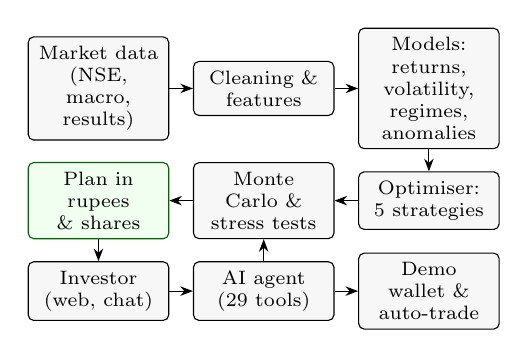
\begin{tikzpicture}[font=\scriptsize, node distance=0.28cm and 0.3cm,
  box/.style={draw, rounded corners=2pt, align=center, minimum height=0.62cm, text width=1.55cm, fill=gray!6},
  hl/.style={box, draw=green!40!black, fill=green!6},
  arr/.style={-{Stealth[length=1.6mm]}, thin}]
  \node[box] (d) {Market data\\(NSE, macro, results)};
  \node[box, right=of d] (c) {Cleaning \&\\features};
  \node[box, right=of c] (m) {Models: returns, volatility, regimes, anomalies};
  \node[box, below=of m] (o) {Optimiser:\\5 strategies};
  \node[box, left=of o] (s) {Monte Carlo \&\\stress tests};
  \node[hl, left=of s] (p) {Plan in rupees \& shares};
  \node[box, below=of s] (a) {AI agent\\(29 tools)};
  \node[box, right=of a] (w) {Demo wallet \&\\auto-trade};
  \node[box, left=of a] (u) {Investor\\(web, chat)};
  \draw[arr] (d) -- (c); \draw[arr] (c) -- (m); \draw[arr] (m) -- (o); \draw[arr] (o) -- (s); \draw[arr] (s) -- (p);
  \draw[arr] (u) -- (a); \draw[arr] (a) -- (s); \draw[arr] (a) -- (w); \draw[arr] (p) -- (u);
\end{tikzpicture}
\caption{System architecture. The language model only selects and explains tools; numbers come from the engine and trading rules are enforced in code.}
\label{fig:arch}
\end{figure}

% =====================================================================
\section{Results}

\subsection{Return prediction}
Table~\ref{tab:lit} compares our models with published results. Measured as an out-of-sample $R^2$ against a zero forecast (the Gu--Kelly--Xiu definition), the price-pattern signal reaches $+0.22\%$, while our fitted Ridge model reaches $-0.24\%$, random forest $-2.43\%$ and XGBoost $-6.46\%$. An $R^2$ of $+0.22\%$ means the signal explains 0.22\% of the month-to-month variation in returns; it is not a 0.22\% return. Its information coefficient on 2021--26 is 0.057 ($t = 2.7$ on independent windows; 0.061, $t = 3.95$, on 2017--20), and it predicts the direction of relative returns correctly 51.5\% of the time against 47.5\% for the historical mean. Five other documented signals (one-week reversal, the MAX effect, idiosyncratic volatility, abnormal volume, low beta) had no skill on 2017--20, nor did post-earnings drift.

\begin{table}[t]
\caption{Our walk-forward results (2021--26) against published work}
\label{tab:lit}
\centering
\setlength{\tabcolsep}{3pt}
\begin{tabular}{@{}p{1.55cm}p{3.15cm}p{3.05cm}@{}}
\toprule
Task & Published & Ours \\
\midrule
Monthly returns, OOS $R^2$ & NN 0.40\%; OLS $-3.46\%$ (US stocks) \cite{gu2020} & Signal $+0.22\%$; Ridge $-0.24\%$ \\
Direction & LSTM 54.3\%, daily, extreme picks, before costs \cite{fischer2018} & 51.5\% monthly, all 32 assets (mean: 47.5\%) \\
Next-month volatility & Forecastable from past volatility \cite{corsi2009} & $R^2$ 0.604 vs 0.503 for the best naive rule \\
Outcome ranges & No common benchmark & 90\% band held 84\% of 104 outcomes \\
\bottomrule
\end{tabular}
\end{table}

\subsection{Volatility forecasting}
On 2021--26 the volatility model reaches $R^2 = 0.604$ on log volatility, against 0.503 for ``same as last quarter'' and 0.388 for ``same as last month''; its average error is 24.6\% against 28.6\% and 30.6\%, and it is ahead of both naive rules in every year (Table~\ref{tab:vol}). Within assets (timing only) $R^2$ is 0.217. Elastic Net, Huber regression, GARCH and implied-volatility features, gradient-boosted trees and LightGBM did not beat it on 2017--20.

How much higher could $R^2$ go? The target, the volatility of 21 fat-tailed daily returns, is itself a noisy measurement. Splitting each window into odd and even days gives two independent measurements of the same month; by the Spearman--Brown formula only 84\% of the target's variation is true volatility for all assets and 63\% for single stocks, which bounds the $R^2$ of any forecaster. Against a cleaner range-based measure of the same 21 days, our stock forecasts score 0.36 instead of 0.28, the effect described by Andersen and Bollerslev \cite{andersen1998}.

\begin{table}[t]
\caption{Volatility forecasts by year: $R^2$ on log volatility (rows with a full 63-day look-ahead)}
\label{tab:vol}
\centering
\begin{tabular}{@{}lccc@{}}
\toprule
Year & Model & Same as last quarter & Same as last month \\
\midrule
2021 & \textbf{0.622} & 0.521 & 0.440 \\
2022 & \textbf{0.517} & 0.465 & 0.338 \\
2023 & \textbf{0.475} & 0.454 & 0.274 \\
2024 & \textbf{0.442} & 0.241 & $-0.046$ \\
2025 & \textbf{0.655} & 0.581 & 0.459 \\
2026 & \textbf{0.584} & 0.274 & 0.277 \\
\bottomrule
\end{tabular}
\end{table}

\subsection{Calibration of the Monte Carlo}
At each quarter-end from 2019 to 2025 the full pipeline was rebuilt from data available at that date and a one-year simulation was run for four portfolios (NIFTY ETF, gold, a 60/20/20 balanced mix and eight large stocks), giving 104 real outcomes. The 50/75/90/95/99\% bands held 49/74/84/89/100\% of them (Fig.~\ref{fig:cal}). Because the outcomes come from overlapping one-year windows of portfolios that move together, we bootstrap whole years of origin dates: the coverage of the 90\% band lies between 72\% and 94\%, so 90\% is plausible but not established. The misses are about location rather than width: 8 of the 17 are gold, which beat its expected return by 17\% a year in 2019--25, and 7 are the rebound after the 2020 crash; without gold the band held 88\%. Earlier periods show the opposite error: on 2016--18 origins the same bands held 98\% of outcomes, and on 2009--17 NIFTY origins 100\%. Wider bands and recentring on past forecast errors were tested with the interval score \cite{gneiting2007}, which penalises both misses and width; neither improved it on pre-2019 data, so the simulator was not changed.

\begin{figure}[t]
\centering
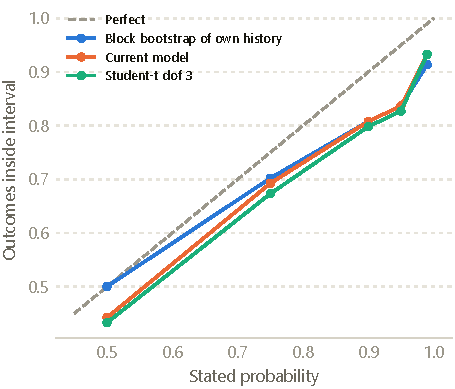
\includegraphics[width=0.78\columnwidth]{eval_calibration.pdf}
\caption{Calibration of one-year Monte Carlo forecasts (104 outcomes, 2019--25). ``Round 5'' is the simulator without volatility uncertainty.}
\label{fig:cal}
\end{figure}

\subsection{Portfolio backtest}
Every month-end from January 2021 the risk model, volatility model, return signal and regime model were rebuilt from data up to that date, weights were optimised under the medium-risk caps, and trades were made at the close with realistic NSE costs per asset class: securities transaction tax, stamp duty, exchange and SEBI fees with GST, and half the bid--ask spread (about 0.17\% to buy and 0.15\% to sell a stock, 0.06\% for equity ETFs). Table~\ref{tab:bt} and Fig.~\ref{fig:curves} show the results. In the max-Sharpe family the volatility model lifts the Sharpe ratio from 0.54 to 0.73, the return tilt to 0.80, and the regime overlay keeps 0.80 while cutting the maximum drawdown from $-16.2\%$ to $-12.2\%$. The NIFTY 50 ETF reaches 0.36. An equal-weight basket of the 26 stocks (0.84) matches the full system.

\begin{table}[t]
\caption{Monthly walk-forward backtest, Jan 2021 -- Oct 2026, realistic costs}
\label{tab:bt}
\centering
\footnotesize
\setlength{\tabcolsep}{3pt}
\begin{tabular}{@{}lccccc@{}}
\toprule
Strategy & CAGR & Vol. & Sharpe & Max DD & Turn. \\
\midrule
Min-variance & 11.5\% & 5.7\% & 0.95 & $-7.0\%$ & 0.8$\times$ \\
\quad + volatility model & 11.1\% & 5.4\% & 0.95 & $-6.0\%$ & 2.7$\times$ \\
Max-Sharpe (prior) & 12.2\% & 11.5\% & 0.54 & $-16.7\%$ & 3.3$\times$ \\
\quad + volatility model & 14.3\% & 11.4\% & 0.73 & $-14.9\%$ & 4.7$\times$ \\
\quad + return tilt & 14.4\% & 10.4\% & 0.80 & $-16.2\%$ & 7.5$\times$ \\
\quad + regime overlay & 13.0\% & 8.6\% & \textbf{0.80} & $-12.2\%$ & 7.4$\times$ \\
\midrule
NIFTY 50 ETF & 10.6\% & 12.8\% & 0.36 & $-16.1\%$ & -- \\
Equal-weight stocks & 16.9\% & 13.0\% & 0.84 & $-15.1\%$ & 0.7$\times$ \\
\bottomrule
\end{tabular}
\end{table}

\begin{figure}[t]
\centering
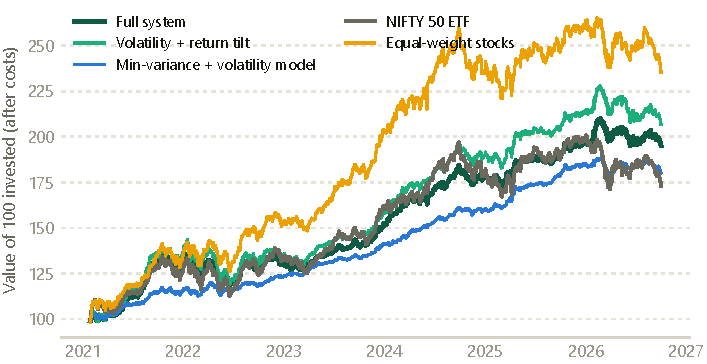
\includegraphics[width=\columnwidth]{eval_curves.pdf}
\caption{Growth of 100 invested, after costs, January 2021 to October 2026.}
\label{fig:curves}
\end{figure}

\subsection{Robustness}
Extending the walk-forward to January 2017 -- October 2026 (117 rebalances; 2017--20 were the selection years, so they are not a clean test), the full system beats the NIFTY ETF in every two-year period (Fig.~\ref{fig:robust}). Over 2017--26 its Sharpe ratio is 0.84 against 0.41, and a stationary block bootstrap \cite{politis1994} of daily returns puts the difference at $+0.43$ with a 90\% interval of $+0.01$ to $+0.83$. Doubling the trading costs lowers the full system's 2021--26 Sharpe ratio by 0.11, and the fixed depository charge per security sold costs a Rs~1 lakh account rebalanced monthly up to 0.15. Two results are weaker than the headline. The volatility model's gain in the max-Sharpe family ($+0.07$ over 2017--26) has a 90\% interval that includes zero, and moving the start of the 2021--26 window by one month moves a strategy's Sharpe ratio by about 0.1. The app's five strategies, chosen at 26 to 34 quarter-ends since 2017 and held with quarterly rebalancing, lost far less than the ETF in their worst year ($+2\%$ for the Goal-Based plan against $-21\%$), but over three years only Max Return clearly beat it on return; the Goal-Based plan did so in 35\% of the windows.

\begin{figure}[t]
\centering
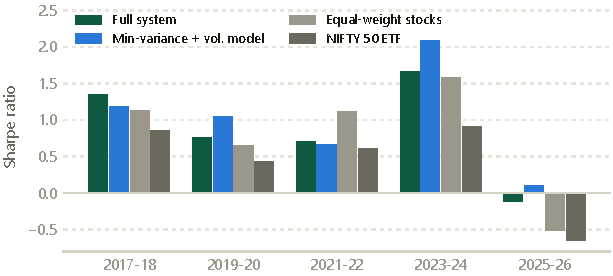
\includegraphics[width=\columnwidth]{robustness.pdf}
\caption{Sharpe ratio by period, walk-forward 2017--26 with realistic costs (2025--26 runs to October 2026).}
\label{fig:robust}
\end{figure}

\subsection{Case study}
For an investor with Rs~1,00,000, a three-year horizon, medium risk and a 12\% target, the engine recommends the Goal-Based plan: an expected return of 14.0\% with 11.6\% volatility, a 53\% probability of reaching the target, a 92\% probability of a gain, a median final value of Rs~1.43 lakh (5th--95th percentile Rs~0.92--2.19 lakh), and survival of 8 of 9 stress tests (Fig.~\ref{fig:dist}). Chosen with data up to October 2023 and held to October 2026, the same strategy returned 55\% against 15\% for the NIFTY 50 index; the robustness analysis above shows that this window was a favourable one.

\begin{figure}[t]
\centering
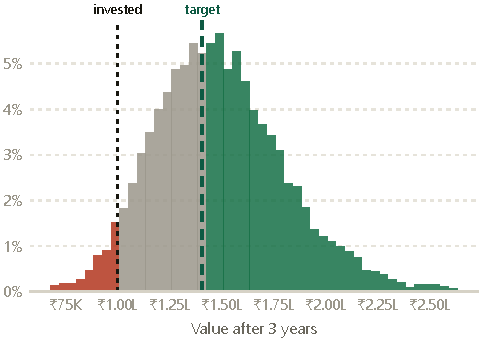
\includegraphics[width=0.9\columnwidth]{distribution.pdf}
\caption{Simulated value after three years for the sample investor (Rs 1 lakh, Goal-Based plan). Green: target met; grey: gain below target; red: loss.}
\label{fig:dist}
\end{figure}

% =====================================================================
\section{Discussion and Limitations}
The system's value lies in risk modelling, not in return forecasting. Volatility is forecastable and improves risk-adjusted performance; returns are barely forecastable, so the signal receives only a 29\% weight and its net contribution is small. In the deployed planner the volatility forecast reports next-month risk, while plans held for one to five years use the long-run Ledoit--Wolf covariance; the monthly-rebalanced backtest uses the forecast to scale the covariance. The main limitations are: (i) the 2021--26 results were inspected over several model-search rounds, so they carry some selection bias, and only a frozen forward test can remove it; (ii) 12 years contain few independent market regimes, and a five-year Sharpe ratio is sensitive to the start date; (iii) the probability of reaching a target depends on expected-return assumptions that are hard to estimate; (iv) the demo wallet charges a flat 0.10\% per trade rather than the per-asset costs used in the backtests; (v) taxes are not modelled. The system is a simulation with demo money and is not investment advice.

% =====================================================================
\section{Conclusion}
\emph{If I Invest Tomorrow} turns an investor's profile into a whole-share plan for the next trading day, together with the probability of reaching the goal, the range of outcomes and the loss in a crash, and lets the investor act on it through a tool-grounded AI agent. Its models are validated walk-forward with rules fixed in advance, and the paper reports the weaker findings alongside the strong ones. Future work includes per-asset trading costs and taxes in the demo wallet, a prospective test of the frozen models, news sentiment, mutual funds and larger local language models.

% =====================================================================
\begin{thebibliography}{00}
\bibitem{markowitz1952} H. Markowitz, ``Portfolio selection,'' \emph{J. Finance}, vol. 7, no. 1, pp. 77--91, 1952.
\bibitem{sharpe1964} W. F. Sharpe, ``Capital asset prices: A theory of market equilibrium under conditions of risk,'' \emph{J. Finance}, vol. 19, no. 3, pp. 425--442, 1964.
\bibitem{ledoit2004} O. Ledoit and M. Wolf, ``A well-conditioned estimator for large-dimensional covariance matrices,'' \emph{J. Multivariate Anal.}, vol. 88, no. 2, pp. 365--411, 2004.
\bibitem{rockafellar2000} R. T. Rockafellar and S. Uryasev, ``Optimization of conditional value-at-risk,'' \emph{J. Risk}, vol. 2, no. 3, pp. 21--41, 2000.
\bibitem{hamilton1989} J. D. Hamilton, ``A new approach to the economic analysis of nonstationary time series and the business cycle,'' \emph{Econometrica}, vol. 57, no. 2, pp. 357--384, 1989.
\bibitem{glasserman2004} P. Glasserman, \emph{Monte Carlo Methods in Financial Engineering}. New York, NY, USA: Springer, 2004.
\bibitem{gu2020} S. Gu, B. Kelly, and D. Xiu, ``Empirical asset pricing via machine learning,'' \emph{Rev. Financial Stud.}, vol. 33, no. 5, pp. 2223--2273, 2020.
\bibitem{chen2016} T. Chen and C. Guestrin, ``XGBoost: A scalable tree boosting system,'' in \emph{Proc. 22nd ACM SIGKDD Int. Conf. Knowl. Discovery Data Mining}, 2016, pp. 785--794.
\bibitem{fischer2018} T. Fischer and C. Krauss, ``Deep learning with long short-term memory networks for financial market predictions,'' \emph{Eur. J. Oper. Res.}, vol. 270, no. 2, pp. 654--669, 2018.
\bibitem{jegadeesh1990} N. Jegadeesh, ``Evidence of predictable behavior of security returns,'' \emph{J. Finance}, vol. 45, no. 3, pp. 881--898, 1990.
\bibitem{jegadeesh1993} N. Jegadeesh and S. Titman, ``Returns to buying winners and selling losers: Implications for stock market efficiency,'' \emph{J. Finance}, vol. 48, no. 1, pp. 65--91, 1993.
\bibitem{blitz2011} D. Blitz, J. Huij, and M. Martens, ``Residual momentum,'' \emph{J. Empirical Finance}, vol. 18, no. 3, pp. 506--521, 2011.
\bibitem{da2014} Z. Da, Q. Liu, and E. Schaumburg, ``A closer look at the short-term return reversal,'' \emph{Manage. Sci.}, vol. 60, no. 3, pp. 658--674, 2014.
\bibitem{grinold2000} R. C. Grinold and R. N. Kahn, \emph{Active Portfolio Management}, 2nd ed. New York, NY, USA: McGraw-Hill, 2000.
\bibitem{corsi2009} F. Corsi, ``A simple approximate long-memory model of realized volatility,'' \emph{J. Financial Econometrics}, vol. 7, no. 2, pp. 174--196, 2009.
\bibitem{parkinson1980} M. Parkinson, ``The extreme value method for estimating the variance of the rate of return,'' \emph{J. Business}, vol. 53, no. 1, pp. 61--65, 1980.
\bibitem{garman1980} M. B. Garman and M. J. Klass, ``On the estimation of security price volatilities from historical data,'' \emph{J. Business}, vol. 53, no. 1, pp. 67--78, 1980.
\bibitem{rogers1991} L. C. G. Rogers and S. E. Satchell, ``Estimating variance from high, low and closing prices,'' \emph{Ann. Appl. Probab.}, vol. 1, no. 4, pp. 504--512, 1991.
\bibitem{andersen1998} T. G. Andersen and T. Bollerslev, ``Answering the skeptics: Yes, standard volatility models do provide accurate forecasts,'' \emph{Int. Econ. Rev.}, vol. 39, no. 4, pp. 885--905, 1998.
\bibitem{liu2008} F. T. Liu, K. M. Ting, and Z.-H. Zhou, ``Isolation forest,'' in \emph{Proc. 8th IEEE Int. Conf. Data Mining (ICDM)}, 2008, pp. 413--422.
\bibitem{beketov2018} M. Beketov, K. Lehmann, and M. Wittke, ``Robo advisors: Quantitative methods inside the robots,'' \emph{J. Asset Manage.}, vol. 19, pp. 363--370, 2018.
\bibitem{yao2023} S. Yao \emph{et al.}, ``ReAct: Synergizing reasoning and acting in language models,'' in \emph{Proc. Int. Conf. Learn. Represent. (ICLR)}, 2023.
\bibitem{schick2023} T. Schick \emph{et al.}, ``Toolformer: Language models can teach themselves to use tools,'' in \emph{Adv. Neural Inf. Process. Syst. (NeurIPS)}, 2023.
\bibitem{politis1994} D. N. Politis and J. P. Romano, ``The stationary bootstrap,'' \emph{J. Amer. Statist. Assoc.}, vol. 89, no. 428, pp. 1303--1313, 1994.
\bibitem{gneiting2007} T. Gneiting and A. E. Raftery, ``Strictly proper scoring rules, prediction, and estimation,'' \emph{J. Amer. Statist. Assoc.}, vol. 102, no. 477, pp. 359--378, 2007.
\end{thebibliography}

\end{document}
